\documentclass[12pt]{scrartcl}

% packages
\usepackage[
    a4paper, total={18cm, 26cm},
    left=0.75in,
    right=0.75in,
    top=0.75in,
    bottom=0.50in,
    footskip=15pt
]{geometry}
\usepackage{lastpage}
\usepackage{graphicx} % \includegraphics
\usepackage{amsmath, esint} % math
\usepackage{steinmetz} % \phase
\usepackage{import} % \import
\usepackage{esdiff} % \diff
\usepackage{fancyhdr} % header and footer
\usepackage{listings}

\makeatletter
\def\today{%
  \two@digits{\the\day}/%
  \ifcase\month\or%
  01\or 02\or 03\or 04\or 05\or 06\or%
  07\or 08\or 09\or 10\or 11\or 12\fi/%
  \number\year%
}
\makeatother

% configs
\setlength{\parindent}{0pt}

% comandos
\renewcommand{\familydefault}{\sfdefault}
\newcommand{\un}[1]{\;\textrm{#1}}
\newcommand{\logo}{\quad \Rightarrow \quad}
\newcommand{\fase}[1]{\ensuremath{\phase{{#1}^{\circ}}}}

\newcommand*\VF[1]{\mathbf{#1}}
\newcommand*\dif{\mathop{}\!\mathrm{d}}


\begin{document}

\pagestyle{fancy}

\fancyhead{}
\fancyhead[L]{Python Aplicado a Sinais e Sistemas - PET Engenharias}
\fancyhead[R]{Data: \today}
\fancyfoot{}
\fancyfoot[R]{Pág. \thepage \; / \pageref{LastPage}}

\begin{center}
    Aluno: Raphael Henrique Braga Leivas \\[20pt]
    Email: rapha.lei8@gmail.com
\end{center}

\hrule

\section*{Atividade 3 - Capítulo 4}

O código completo usado nessa atividade se encontra no ANEXO A.

\subsection*{Exercício 1}

Usando o software (veja ANEXO A), as transformadas de Laplace pedidas são

\[ 
(a) \,\, \frac{s - 3}{\left(s - 3\right)^{2} + 4} \quad 
(b) \,\, \frac{120}{\left(s - 4\right)^{6}} \quad 
(c) \,\, \frac{5 \left(s^{2} - 11\right)}{\left(s^{2} + 1\right) \left(s^{2} + 121\right)} \quad 
(d) \,\, \frac{1}{s^{2} - 1} 
\]

\subsection*{Exercício 2}

Usando o software (veja ANEXO A), e definindo a função degrau unitário como $\theta (t)$, 
as transformadas inversas são dadas por 

\[ 
(a) \,\,  \frac{e^{3 t} \theta\left(t\right)}{4} - \frac{e^{- t} \theta\left(t\right)}{4} \quad
(b) \,\, \frac{t^{8} \theta\left(t\right)}{896} + \frac{t^{7} \theta\left(t\right)}{1008} 
\]

\[ 
(c) \,\, - \left(\frac{\sqrt{3} e^{\frac{t}{2}} \sin{\left(\frac{\sqrt{3} t}{2} \right)}}{3} + \frac{e^{\frac{t}{2}} \cos{\left(\frac{\sqrt{3} t}{2} \right)}}{3}\right) \theta\left(t\right) + \frac{e^{- t} \theta\left(t\right)}{3} \quad 
\]

\[ 
(d) \,\, \left(- \frac{81 \sqrt{11} \sin{\left(\sqrt{11} t \right)}}{110} + \frac{11 \cos{\left(\sqrt{11} t \right)}}{10}\right) \theta\left(t\right) + \left(\frac{81 \sin{\left(t \right)}}{10} - \frac{\cos{\left(t \right)}}{10}\right) \theta\left(t\right) 
\]

\subsection*{Exercício 3}

Temos uma EDO linear dada por

\[  32 c{\left(t \right)} + 12 \frac{d}{d t} c{\left(t \right)} + \frac{d^{2}}{d t^{2}} c{\left(t \right)} = t^2 \]

Tiramos o Laplace de ambos lados da equação, considerando as condições iniciais nulas

\[  32 C(s) + 12 s C(s) + s^2 C(s) = \frac{2}{s^3} \]

Cuja solução é  

\[ C(s) = \frac{2}{s^{3} \left(s^{2} + 12 s + 32\right)} \]

Tomando a transformada inversa de $C(s)$, obtemos a solução $c(t)$ da EDO:

\[ c(t) = \frac{t^{2} \theta\left(t\right)}{32} - \frac{3 t \theta\left(t\right)}{128} + \frac{7 \theta\left(t\right)}{1024} - \frac{e^{- 4 t} \theta\left(t\right)}{128} + \frac{e^{- 8 t} \theta\left(t\right)}{1024} \]

\subsection*{Exercício 4}

Usando o código do ANEXO A, temos o gráfico de polos e zeros de $C(s)$ do exercício 
anterior exibido abaixo:

\begin{figure}[h!]
	\begin{center}
    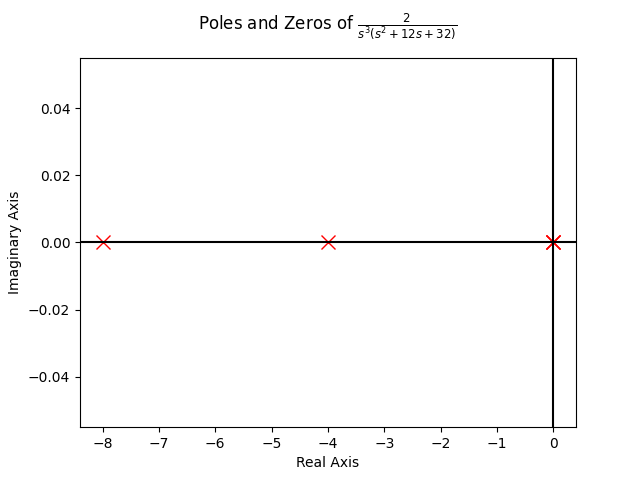
\includegraphics[width=0.8\textwidth,trim=1 1 1 1,clip]{ex4.png}
	\end{center}
\end{figure}

\subsection*{Exercício 5}

Os Diagramas de Bode de $C(s)$ estão exibidos abaixo. Note que a frequência está em Hz 
e a fase em graus.

\begin{figure}[h!]
	\begin{center}
    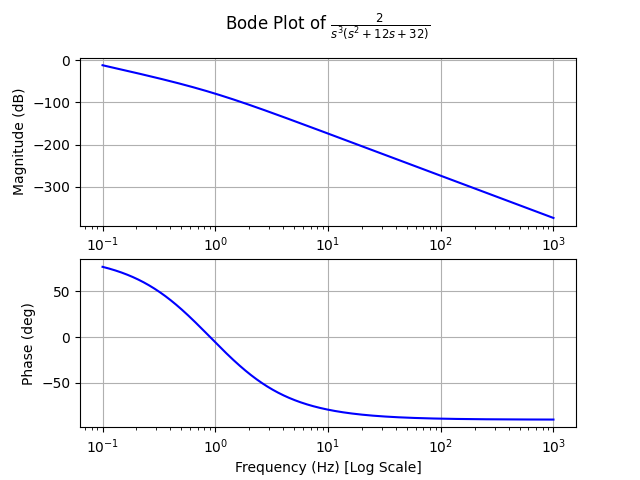
\includegraphics[width=0.8\textwidth,trim=1 1 1 1,clip]{ex5.png}
	\end{center}
\end{figure}

\newpage

\section*{ANEXO A - Código}

\begin{lstlisting}[language=Python, breaklines=true, basicstyle=\scriptsize]
    import numpy as np
    import matplotlib as plt
    from sympy import *
    from sympy.physics.control.control_plots import pole_zero_plot
    from sympy.physics.control.control_plots import bode_plot
    from sympy.physics.control.lti import TransferFunction
    
    ## Exercicio 1
    
    t, s = symbols('t, s')
    funcoes = [exp(3*t) * cos(2*t), t**5 * exp(4*t), sin(5*t) * cos(6*t), sinh(t)]
    
    for f in funcoes:
        print(latex(laplace_transform(f, t, s, noconds=True)))
    
    ## Exercicio 2
    
    print("Ex 2 --------------")
    
    funcoes_inv = [1 / (s**2 - 2*s - 3), (5*s + 45) / s**9, -s / (s**3 + 1), (s**3 + 81) / (s**4 + 12 * s**2 + 11)]
    for f in funcoes_inv:
        print(latex(inverse_laplace_transform(f, s, t, noconds=True)))
    
    ## Exercicio 3
    
    c, C = symbols('c C', cls = Function)
    
    # cond iniciais
    y0 = 0
    dy_0 = 0
    
    eq_s = Eq(32 * C(s) + 12 * s * C(s) + s**2 * C(s), 2 / s**3)
    
    cs_solucao = solve(eq_s, C(s))[0]
    
    print(latex(cs_solucao))
    
    print(latex(inverse_laplace_transform(cs_solucao, s, t, noconds=True)))
    
    ## Exercicio 4
    
    # extrai o numerador e denominador
    num, den = fraction(cs_solucao)
    ft1 = TransferFunction(num, den, s)
    pole_zero_plot(ft1, pole_color="red", grid=False)
    
    ## Exercicio 5
    
    bode_plot(ft1, initial_exp=-1, final_exp=3, phase_unit='deg', freq_unit='Hz')
\end{lstlisting}

\end{document}